\begin{center}
    {\large\bfseries Непрерывная олимпиада. Тур 1}
\end{center}

\footnotesize

\begin{enumerate}

    \item Найдите наибольшее чётное число,
которое делится на 75 и не содержит в
своей записи одинаковых цифр.

\item
\begin{minipage}[c]{0.52\linewidth}
Разрежьте фигуру на трёхклеточные уголки так, чтобы в каждом уголке было
по кружочку.
\end{minipage}\hfill
\begin{minipage}[c]{0.43\linewidth}
\centering
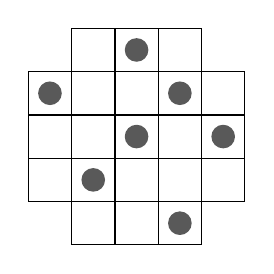
\begin{tikzpicture}[x=0.55cm,y=0.55cm,line width=0.45pt]
    \foreach \x in {1,2,3} {
        \draw (\x,0) rectangle ++(1,-1);
        \draw (\x,-4) rectangle ++(1,-1);
    }
    \foreach \y in {-1,-2,-3} {
        \foreach \x in {0,1,2,3,4} {
            \draw (\x,\y) rectangle ++(1,-1);
        }
    }

    \foreach \p in {(2.5,-0.5),(0.5,-1.5),(3.5,-1.5),
                     (2.5,-2.5),(4.5,-2.5),(1.5,-3.5),(3.5,-4.5)} {
        \fill[black!65] \p circle[radius=0.15cm];
    }
\end{tikzpicture}
\end{minipage}

\item Во фруктовой лавке есть пять дынь
различного веса, каждая весит целое
число килограммов. Две самые тяжёлые
дыни весят в два раза больше остальных
трёх, а три самые тяжёлые дыни весят в
восемь раз больше остальных двух.
Найдите наименьшее возможное
значение суммарного веса всех дынь.

\end{enumerate}
